% Provenance (never printed): see sources/outline_sources.md (Year 1: insolation with
% latitude and season, the radiative surplus and deficit, meridional heat transport by
% the atmosphere and the ocean, latent heat). Exercise and problem values in the Book 3
% scratch calculator calc/ch27.py; figures from figdata/bachelor-1/insolation.py (Kepler
% orbit of _solar.py) and energy_balance.py (NCEP-NCAR Reanalysis 1, long-term means
% 1991-2020, datasets bachelor-1-ncep-*).
% Physics owns the inverse-square law, the black body and the Stefan-Boltzmann law, the
% seasons and latent heat (recalled). Book 2 (g10) gave the quarter of the solar constant,
% the global budget diagram and its closure, latent and sensible heat in words, the
% annual-mean insolation curve and the poleward transport in words: re-founded here with
% derivations and data. Ch. 1 gave the instantaneous insolation, the declination and the
% rising and setting of the Sun.
\chapter{辐射与热量输送}\label{ch:b1:radiation-heat-transport}

从一百万英里外看，被阳光照亮的地球是一个圆盘，
上面有蓝色的海洋、棕色的陆地和白色的云。阳光最为直射的是圆盘中部，
靠近热带的地方，阳光向边缘则掠射。热带吸收的能量
远多于极地地区。然而，热带并没有年复一年
变得更热，极地也没有变得更冷。风和洋流把多余的热量输送向
极地，其量级可达数拍瓦。本章测量这一平衡中的三项：
每个\omterm{def:b1:spherical-astronomy:geographic}{纬度}所接收的阳光、它所保留的部分以及向太空发出的红外辐射，
以及弥补两者差额的输送。输送中有相当大的部分
以不可见的形式进行，即水蒸气，其潜热
在凝结成雨的地方释放出来。
% ledger: commons:epic-earth, trenberth:transport

\begin{omfigure}
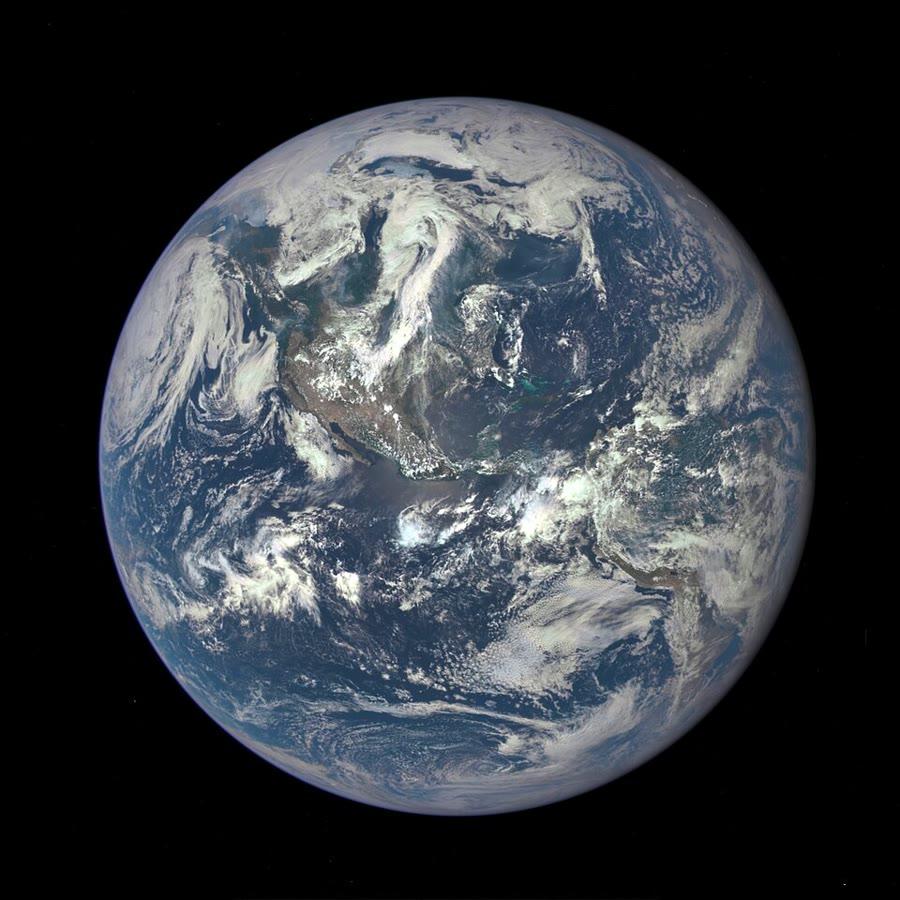
\includegraphics[width=0.55\linewidth]{images/book3/b1-epic-earth.jpg}

{\small 地球被阳光照亮的一面的全景，2015 年 7 月 6 日由深空气候观测站上的
照相机拍摄，距离一百万英里；北美洲和中美洲位于画面中央，
加勒比海浅水区呈绿松石色。夏至后两周，位于画面顶部的北极圈
整日都被照亮。明亮的云层反射了照到它们上面的大部分光线；
带蓝色的色调来自
空气分子对阳光的散射。（NASA 戈达德太空飞行中心，
公有领域，经由维基共享资源。）}
\label{fig:b1:radiation-heat-transport:epic}
\end{omfigure}
% ledger: commons:epic-earth (polar day: figdata/bachelor-1/insolation.py)

\begin{recall}
\Cref{ch:b1:spherical-astronomy}中定义了\omterm{def:b1:spherical-astronomy:insolation}{日射量}，即大气层顶部水平面上每平方米
接收的太阳光功率，
在太阳位于地平线以上时，$I = S_0(a/r)^2\sin h_\odot$，其中 $S_0 = \qty{1361}{W.m^{-2}}$
为平均距离 $a$ 处的值；给出了太阳高度角由\omterm{def:b1:spherical-astronomy:equatorial}{时角} $H$、
\omterm{def:b1:spherical-astronomy:equatorial}{赤纬} $\delta$ 和\omterm{def:b1:spherical-astronomy:geographic}{纬度} $\varphi$ 确定的关系，
$\sin h_\odot = \sin\varphi\sin\delta + \cos\varphi\cos\delta\cos H$；并给出了日落\omterm{def:b1:spherical-astronomy:equatorial}{时角}
$H_0$ 的公式，$\cos H_0 = -\tan\varphi\tan\delta$
（\cref{prop:b1:spherical-astronomy:rising}）。\Cref{ch:b1:comparative-planetology}
中定义了行星的\omterm{def:b1:comparative-planetology:albedo}{邦德反照率}及其\omterm{def:b1:comparative-planetology:equilibrium-temperature}{平衡温度}。物理学分册给出了光的平方反比律、
黑体辐射的 $\sigma T^4$ 公式（每平方米，$\sigma = \qty{5.670e-8}{W.m^{-2}.K^{-4}}$，
即斯特藩–玻尔兹曼定律），以及相变的潜热。第 2 册指出，地球平均
截获太阳常数的四分之一，
画出了地球的全球能量收支图，
并验证其收支平衡，
又以文字描述了热量向极地的输送。
% ledger: earth:TSI, const:sigma, ipcc:budget-toa
\end{recall}

\section{日射量随纬度和季节的变化}\label{sec:b1:radiation-heat-transport:insolation}

瞬时\omterm{def:b1:spherical-astronomy:insolation}{日射量}随太阳在天空中运动而每时每刻变化。
对于气候而言，关心的是其一日之内的总和。

\begin{definition}[日平均日射量]\label{def:b1:radiation-heat-transport:daily-insolation}
某一\omterm{def:b1:spherical-astronomy:geographic}{纬度}在某一天的\emph{日平均日射量}\index{日平均日射量} $\bar Q$，
是该日 24 小时（包括夜间）内瞬时\omterm{def:b1:spherical-astronomy:insolation}{日射量}的平均值，
其中太阳\omterm{def:b1:spherical-astronomy:equatorial}{赤纬}和日地距离取该日的数值并保持不变。它是大气层顶部水平面上的
每平方米的功率，
单位为 \unit{W.m^{-2}}。
\end{definition}

在一天之内保持 $\delta$ 和 $r$ 不变是无妨的：\omterm{def:b1:spherical-astronomy:equatorial}{赤纬}每天的变化
至多为 \ang{0.4}，日地距离的变化小于 \qty{0.03}{\percent}。
% ledger: earth:obliquity, earth:ecc (computed in figdata/bachelor-1/insolation.py)

\begin{theorem}[日平均日射量]\label{thm:b1:radiation-heat-transport:daily}
设\omterm{def:b1:spherical-astronomy:geographic}{纬度}为 $\varphi$，某日太阳\omterm{def:b1:spherical-astronomy:equatorial}{赤纬}为 $\delta$，
日地距离为 $r$，则
\[
  \bar Q = \frac{S_0}{\pi}\left(\frac{a}{r}\right)^{2}
  \bigl(h_0\sin\varphi\sin\delta + \cos\varphi\cos\delta\sin h_0\bigr),
\]
其中 $h_0 \in [0, \pi]$ 为以弧度计的日落\omterm{def:b1:spherical-astronomy:equatorial}{时角}：$\cos h_0 =
-\tan\varphi\tan\delta$（当 $|\tan\varphi\tan\delta| \le 1$ 时）；$h_0 = \pi$ 对应
极昼（$\tan\varphi\tan\delta > 1$）；$h_0 = 0$ 且 $\bar Q = 0$ 对应
极夜（$\tan\varphi\tan\delta < -1$）。
\end{theorem}

\begin{proof}
\omterm{def:b1:spherical-astronomy:equatorial}{时角} $H$ 在一天之内匀速变化 $2\pi$，故一日的平均值
即为 $H \in [-\pi, \pi]$ 上的平均值。太阳在 $-h_0 < H < h_0$ 时位于地平线以上，
此时 $\sin h_\odot > 0$，其余时间\omterm{def:b1:spherical-astronomy:insolation}{日射量}为零。于是
\[
  \bar Q = \frac{1}{2\pi}\int_{-h_0}^{h_0} S_0\left(\frac{a}{r}\right)^{2}
  \bigl(\sin\varphi\sin\delta + \cos\varphi\cos\delta\cos H\bigr)\,\mathrm dH ,
\]
即为 $(S_0/2\pi)(a/r)^2\bigl(2h_0\sin\varphi\sin\delta +
2\cos\varphi\cos\delta\sin h_0\bigr)$。
积分上下限由\cref{prop:b1:spherical-astronomy:rising}得出：高度角为零时
即 $\cos H = -\tan\varphi\tan\delta$。若该数的绝对值大于 1，
则太阳永不穿越地平线：当 $\tan\varphi\tan\delta > 1$ 时，
被积函数对所有 $H$ 均为正，积分遍及整日，
$h_0 = \pi$；当 $\tan\varphi\tan\delta < -1$ 时，被积函数对所有 $H$ 均为负，
太阳永不升起。
\end{proof}

有两种特殊情形值得牢记。在赤道上，$\varphi = 0$，
无论季节如何，$h_0 = \pi/2$：
\[
  \bar Q_\text{赤道} = \frac{S_0}{\pi}\left(\frac{a}{r}\right)^{2}\cos\delta ,
\]
在春分和秋分时最大，平均距离处其值为 $S_0/\pi = \qty{433.2}{W.m^{-2}}$。
在极点的夏季，$h_0 = \pi$ 且 $\varphi = \pi/2$：$\bar Q_\text{极} =
S_0(a/r)^2\sin\delta$，此时太阳在天空中以
等于\omterm{def:b1:spherical-astronomy:equatorial}{赤纬}的恒定高度环绕运行。
% ledger: earth:TSI

\begin{proposition}[极地夏季]\label{prop:b1:radiation-heat-transport:polar-summer}
在\omterm{def:b1:spherical-astronomy:equatorial}{赤纬} $\delta > 0$ 的某日，北极的\omterm{def:b1:radiation-heat-transport:daily-insolation}{日平均日射量}
超过赤道，当且仅当 $\pi\tan\delta > 1$，即 $\delta >
\ang{17.66}$。在六月至日，$\delta = \ang{23.44}$，此时比值为 $\pi\tan
\delta = 1.362$。
\end{proposition}

\begin{proof}
上述两种特殊情形有共同的因子 $(S_0/\pi)(a/r)^2$；二者之比为
$\pi\sin\delta/\cos\delta = \pi\tan\delta$，当 $\tan\delta >
1/\pi$，即 $\delta > \arctan(1/\pi) = \ang{17.66}$ 时，该比值大于 1。计入\omterm{def:b1:spherical-astronomy:ecliptic}{黄赤交角}后，
$\pi\tan\ang{23.44} = 1.362$。
\end{proof}
% ledger: earth:obliquity

考虑地球轨道，六月至日接近远日点，$(a/r)^2 = 0.968$：
此时北极日平均接收 \qty{524}{W.m^{-2}}，赤道为
\qty{385}{W.m^{-2}}。六个月之后，南极接近近日点，接收
\qty{559}{W.m^{-2}}，比北极夏季时多 \qty{6.7}{\percent}，
二者之比恰等于两个 $(a/r)^2$ 值之比。下图给出一整年中的 $\bar Q$。
极大值出现在两极的至日；深色楔形区为极夜，
其边界\omterm{def:b1:spherical-astronomy:geographic}{纬度}为 $\ang{90} -
|\delta|$；太阳直射点即正午太阳经过头顶之处，
其位置随\omterm{def:b1:spherical-astronomy:equatorial}{赤纬}在回归线之间移动。
% ledger: earth:TSI, earth:ecc, earth:obliquity, nasa:earth-perihelion-longitude, usno:seasons-2026 (computed in figdata/bachelor-1/insolation.py)

\begin{omfigure}
\begin{tikzpicture}
\begin{axis}[omrecord, width=0.8\linewidth, height=6.4cm, view={0}{90},
  xmin=0, xmax=365, ymin=-90, ymax=90, xlabel={一年中的日序（自 1 月 1 日起）},
  ylabel={纬度 (\unit{\degree})}, xtick={0,60,...,360}, ytick={-90,-60,...,90},
  colormap/viridis, colorbar, point meta min=0, point meta max=560,
  colorbar style={ylabel={$\bar Q$ (\unit{W.m^{-2}})}, ytick={0,100,...,500}, width=0.3cm},
  axis on top, grid=none]
% figdata/bachelor-1/insolation.py; ledger: earth:TSI, earth:ecc, earth:obliquity, nasa:earth-perihelion-longitude, usno:tropical-year, usno:seasons-2026
\addplot3[surf, shader=interp, mesh/ordering=y varies, mesh/rows=73]
  table[x=day, y=lat, z=Q] {figdata/out/bachelor-1-insolation-grid.dat};
\addplot3[white, dashed, line width=0.8pt] table[x=day, y=decl, z expr=600] {figdata/out/bachelor-1-insolation-sun.dat};
\addplot3[white, line width=0.6pt, unbounded coords=jump] table[x=day, y=night_n, z expr=600] {figdata/out/bachelor-1-insolation-sun.dat};
\addplot3[white, line width=0.6pt, unbounded coords=jump] table[x=day, y=night_s, z expr=600] {figdata/out/bachelor-1-insolation-sun.dat};
\node[font=\scriptsize, text=white] at (axis cs:28,81,700) {极夜};
\node[font=\scriptsize, text=white] at (axis cs:172,-81,700) {极夜};
\node[font=\scriptsize, text=white, anchor=south] at (axis cs:172,26,700) {太阳直射纬度};
\end{axis}
\end{tikzpicture}

{\small 大气层顶的\omterm{def:b1:radiation-heat-transport:daily-insolation}{日平均日射量}随一年中的日序与\omterm{def:b1:spherical-astronomy:geographic}{纬度}的变化，
取自 \cref{thm:b1:radiation-heat-transport:daily}，其中
$S_0 = \qty{1361}{W.m^{-2}}$，并计入地球轨道。虚线：太阳直射\omterm{def:b1:spherical-astronomy:geographic}{纬度}，
等于\omterm{def:b1:spherical-astronomy:equatorial}{赤纬}；实线：极夜的边界。夏季极地接收的\omterm{def:b1:spherical-astronomy:insolation}{日射量}
高于地球上任何其他地方；南半球夏季接近
近日点，是两者中更亮的一个。}
\label{fig:b1:radiation-heat-transport:matrix}
\end{omfigure}
% ledger: earth:TSI, earth:ecc, earth:obliquity, nasa:earth-perihelion-longitude, usno:seasons-2026

对 $\bar Q$ 作全年平均，得到各\omterm{def:b1:spherical-astronomy:geographic}{纬度}的年平均\omterm{def:b1:spherical-astronomy:insolation}{日射量}
（见下图）：赤道为 \qty{415.6}{W.m^{-2}}，\ang{40} 处为 \qty{328.3}{W.m^{-2}}，
两极各为 \qty{172.4}{W.m^{-2}}。极地夏季的日射强烈，
但极地冬季黑暗，全年赤道接收的\omterm{def:b1:spherical-astronomy:insolation}{日射量}是极点的 \num{2.41} 倍。
两个半球的曲线相同，尽管南半球夏季更亮；
\cref{exo:b1:radiation-heat-transport:10} 说明了其原因。
% ledger: earth:TSI, earth:ecc, earth:obliquity (computed in figdata/bachelor-1/insolation.py)

\begin{omfigure}
\begin{tikzpicture}
\begin{axis}[omrecord, width=0.8\linewidth, height=5.6cm, xmin=-90, xmax=90, ymin=0, ymax=600,
  xlabel={纬度 (\unit{\degree})}, ylabel={$\bar Q$ (\unit{W.m^{-2}})},
  xtick={-90,-60,...,90}, ytick={0,100,...,600}]
% figdata/bachelor-1/insolation.py; ledger: earth:TSI, earth:ecc, earth:obliquity, nasa:earth-perihelion-longitude
\addplot[omThm, line width=0.8pt] table[x=lat, y=Q_jun] {figdata/out/bachelor-1-insolation-annual.dat};
\addplot[omDef, line width=0.8pt] table[x=lat, y=Q_dec] {figdata/out/bachelor-1-insolation-annual.dat};
\addplot[black, line width=1.1pt] table[x=lat, y=Q_ann] {figdata/out/bachelor-1-insolation-annual.dat};
\addplot[black!60, dashed, domain=-90:90] {340.30};
\node[font=\scriptsize, text=omThm, anchor=west] at (axis cs:50,540) {六月至日};
\node[font=\scriptsize, text=omDef, anchor=east] at (axis cs:-50,575) {十二月至日};
\node[font=\scriptsize, anchor=north] at (axis cs:-72,160) {年平均};
\node[font=\scriptsize, text=black!60, anchor=south west] at (axis cs:-88,342) {全球平均};
\end{axis}
\end{tikzpicture}

{\small 两个至日的\omterm{def:b1:radiation-heat-transport:daily-insolation}{日平均日射量}随\omterm{def:b1:spherical-astronomy:geographic}{纬度}的变化，以及其年平均（黑线）。
年平均超过全球平均值 \qty{340.3}{W.m^{-2}}，
（虚线）的范围为南纬 \ang{37} 至北纬 \ang{37}，
占地球表面的 \qty{60}{\percent}。}
\label{fig:b1:radiation-heat-transport:annual}
\end{omfigure}
% ledger: earth:TSI, earth:ecc, earth:obliquity (computed in figdata/bachelor-1/insolation.py)

\begin{proposition}[全球平均]\label{prop:b1:radiation-heat-transport:global}
在任一时刻，对整个球面平均的\omterm{def:b1:spherical-astronomy:insolation}{日射量}为 $\tfrac14
S_0(a/r)^2$。若再对一年取平均，则为 $S_0/(4\sqrt{1 - e^2})$，其中
$e$ 为轨道的偏心率：对地球而言为 \qty{340.30}{W.m^{-2}}，
与 $S_0/4 = \qty{340.25}{W.m^{-2}}$ 相差不超过 \qty{0.02}{\percent}。
\end{proposition}

\begin{proof}
半径为 $R$ 的地球截获穿过面积为 $\pi
R^2$ 圆盘的阳光，功率为 $S_0(a/r)^2\pi R^2$，落在白昼半球上；
将其均摊到整个表面 $4\pi R^2$ 上，即得第一个结果。$(a/r)^2$ 的时间平均
在轨道上为 $1/\sqrt{1-e^2}$
（见\cref{exo:b1:radiation-heat-transport:11}）。
\end{proof}
% ledger: earth:TSI, earth:ecc

\section{吸收与发射的辐射}\label{sec:b1:radiation-heat-transport:toa}

某\omterm{def:b1:spherical-astronomy:geographic}{纬度}所接收的太阳光中，一部分被直接反射回去，
反射来源包括云、雪、冰、沙漠，以及程度稍小的海；其余部分则被
空气和地表吸收。地球还通过
昼夜不停地向太空发射红外线而损失能量。

\begin{definition}[向外长波辐射]\label{def:b1:radiation-heat-transport:olr}
称\emph{向外长波辐射}\index{向外长波辐射}（OLR）为
从大气顶部射向太空的红外辐射功率，
按每平方米计。\emph{发射温度}\index{发射温度}
$T_e$ 是一个黑体的温度，该黑体发射的功率与之相同：
$\sigma T_e^4 = \text{OLR}$。
\end{definition}

OLR 一部分来自地表，穿过对红外线透明的空气射出；
另一部分来自较高处的空气与云顶。\omterm{def:b1:radiation-heat-transport:olr}{发射
温度}是辐射本身的性质，而非某一层的温度：
它低于下方地面的温度，
因为发射层较冷。
% ledger: ipcc:budget-surface, ipcc:budget-toa

\begin{definition}[净辐射；辐射盈余与亏损]\label{def:b1:radiation-heat-transport:net-radiation}
大气顶部的\emph{净辐射}\index{净辐射}为
\[
  R = \underbrace{(1 - \alpha)\,\bar Q}_{\text{吸收的太阳辐射}} - \text{OLR},
\]
其中 $\alpha$ 为局地反照率，即入射太阳光中被反射回太空的比例；
三个量均为某一\omterm{def:b1:spherical-astronomy:geographic}{纬度}的年平均值。
$R > 0$ 的\omterm{def:b1:spherical-astronomy:geographic}{纬度}具有\emph{辐射盈余}\index{辐射盈余}；$R < 0$ 的\omterm{def:b1:spherical-astronomy:geographic}{纬度}
具有\emph{辐射亏损}\index{辐射亏损}。
\end{definition}

就整个地球而言，\omterm{def:b1:radiation-heat-transport:net-radiation}{净辐射}的全球平均值必须接近零，因为行星
其升温或降温的幅度每平方米都不超过零点几瓦特：
最新评估给出的失衡量为 \qty{0.7}{W.m^{-2}}，入射
\qty{340}{W.m^{-2}} 中有 \qty{100}{W.m^{-2}} 被反射（全球反照率为
\num{0.294}），\qty{239}{W.m^{-2}} 以红外线形式离开。
% ledger: ipcc:budget-toa, earth:albedo

本章的纬向剖面取自再分析资料，即用过去数十年的天气预报系统
重新运行得到的数据集，该系统同化
每日观测，并输出完整且自洽的大气状态。
这里所用的再分析资料始于 1948 年，给出的是月平均值，网格为 94 个\omterm{def:b1:spherical-astronomy:geographic}{纬度}、
192 个\omterm{def:b1:spherical-astronomy:geographic}{经度}；本章取其 1991--2020 年的平均值。其辐射
通量是模式输出，即受观测约束的预报。下图
给出其纬向平均值，横轴为 $\sin\varphi$，因此横轴上
等长的区间对应球面上等面积的区域。
% ledger: psl:ncep-r1, kalnay96:reanalysis, data:b3-ncep

\begin{omfigure}
\begin{tikzpicture}
\begin{axis}[omrecord, width=0.8\linewidth, height=6cm, xmin=-1, xmax=1, ymin=0, ymax=320,
  xlabel={纬度（\unit{\degree}，横轴为 $\sin\varphi$）}, ylabel={通量（\unit{W.m^{-2}}）},
  xtick={-0.866,-0.5,0,0.5,0.866}, xticklabels={60 南, 30 南, 0,30 北, 60 北},
  ytick={0,50,...,300}]
% figdata/bachelor-1/energy_balance.py; ledger: data:b3-ncep, psl:ncep-r1
\addplot[name path=asr, omProp, line width=1pt] table[x expr={sin(\thisrow{lat})}, y=asr] {figdata/out/bachelor-1-energy_balance-toa.dat};
\addplot[name path=olr, omThm, line width=1pt] table[x expr={sin(\thisrow{lat})}, y=olr] {figdata/out/bachelor-1-energy_balance-toa.dat};
\addplot[omProp!25] fill between[of=asr and olr, split, every segment no 1/.style={omDef!18}, every segment no 2/.style={omProp!30}, every segment no 3/.style={omDef!18}];
\node[font=\scriptsize, text=omProp!80!black] at (axis cs:-0.55,300) {吸收的太阳辐射};
\node[font=\scriptsize, text=omThm] at (axis cs:-0.2,226) {OLR};
\node[font=\scriptsize] at (axis cs:0,262) {盈余};
\node[font=\scriptsize] at (axis cs:0.86,178) {亏损};
\node[font=\scriptsize] at (axis cs:-0.86,178) {亏损};
\end{axis}
\end{tikzpicture}

{\small 大气顶部吸收的太阳辐射（橙色）与\omterm{def:b1:radiation-heat-transport:olr}{向外长波辐射}（红色）的纬向及年平均值，
取自 NCEP-NCAR Reanalysis~1，
平均时段为 1991--2020 年（数据由 NOAA PSL 提供，
位于美国科罗拉多州博尔德市，网址 https://psl.noaa.gov）。阴影部分：低\omterm{def:b1:spherical-astronomy:geographic}{纬度}的
\omterm{def:b1:radiation-heat-transport:net-radiation}{辐射盈余}与高\omterm{def:b1:spherical-astronomy:geographic}{纬度}的\omterm{def:b1:radiation-heat-transport:net-radiation}{辐射亏损}。}
\label{fig:b1:radiation-heat-transport:toa}
\end{omfigure}
% ledger: data:b3-ncep, psl:ncep-r1, kalnay96:reanalysis

两条曲线的形状差异很大。吸收的太阳光从
赤道附近的 \qty{288}{W.m^{-2}} 降至北纬 \ang{81} 处的 \qty{76}{W.m^{-2}}，下降为
原来的 \num{3.8} 分之一：\omterm{def:b1:spherical-astronomy:insolation}{日射量}减小，反照率则由 \num{0.31} 升至
\num{0.57}，原因在于太阳高度角低，且有积雪与海冰。OLR 仅从
\qty{245}{W.m^{-2}} 降至 \qty{192}{W.m^{-2}}，下降为原来的 \num{1.27} 分之一；
\omterm{def:b1:radiation-heat-transport:olr}{发射温度}分别为 \qty{256}{K} 与 \qty{241}{K}。赤道处的 OLR 甚至
略低，为 \qty{245}{W.m^{-2}}，低于北纬 \ang{20} 处的 \qty{269}{W.m^{-2}}：
赤道降雨带的云层高耸，其冷的云顶发射的辐射很少，
而较为晴朗的副热带天空使更多红外线逸出。凡吸收的太阳光超过 OLR 之处，
该\omterm{def:b1:spherical-astronomy:geographic}{纬度}即具有盈余。
% ledger: data:b3-ncep (values computed in figdata/bachelor-1/energy_balance.py)

\begin{example}[再分析资料的全球收支]\label{ex:b1:radiation-heat-transport:global}
对全球取平均，再分析资料给出的入射辐射为 \qty{341.9}{W.m^{-2}}，
反射 \qty{117.0}{W.m^{-2}}（反照率为 \num{0.342}），吸收 \qty{224.8}{W.m^{-2}}，
发射 \qty{237.7}{W.m^{-2}}：\omterm{def:b1:radiation-heat-transport:net-radiation}{净辐射}为 \qty{-12.9}{W.m^{-2}}。OLR 与评估值
\qty{239}{W.m^{-2}} 相差在 \qty{1.3}{W.m^{-2}} 以内，但反射量
比评估值 \qty{100}{W.m^{-2}} 大 \qty{17}{W.m^{-2}}。若真实
失衡量达到此量级，地球将以 \qty{6.6}{PW} 的速率降温；这是模式的误差，
并非地球的性质，下文的输运量是在去除
全球平均值之后计算的。
% ledger: data:b3-ncep, ipcc:budget-toa (computed in figdata/bachelor-1/energy_balance.py)
\end{example}

\section{经向热量输送}\label{sec:b1:radiation-heat-transport:transport}

\begin{definition}[经向热量输送]\label{def:b1:radiation-heat-transport:mht}
称\emph{经向热量输送}\index{经向热量输送} $T(\varphi)$ 为
单位时间内穿过纬线 $\varphi$ 向北输送的能量，
由大气与海洋共同输送，取年平均值。
规定向北为正，并以拍瓦为单位。
（\qty{1}{PW} = \qty{e15}{W}）。
\end{definition}

\begin{proposition}[由净辐射得到的输运]\label{prop:b1:radiation-heat-transport:mht}
若每一\omterm{def:b1:spherical-astronomy:geographic}{纬度}带所储存的能量逐年不变，则
对于半径为 $a_\oplus$ 的地球，
\[
  T(\varphi) = 2\pi a_\oplus^2\int_{-\pi/2}^{\varphi} R(\varphi')\cos\varphi'\,
  \mathrm d\varphi' = -2\pi a_\oplus^2\int_{\varphi}^{\pi/2} R(\varphi')\cos
  \varphi'\,\mathrm d\varphi' ,
\]
且 $T$ 在 $R$ 变号的\omterm{def:b1:spherical-astronomy:geographic}{纬度}处取极值。
\end{proposition}

\begin{proof}
取位于纬线 $\varphi$ 以南的极冠作为控制体，从
海洋底部到大气顶部（见下图）。能量只能通过两种方式进出该控制体：
在顶部以辐射形式进出，净功率为
$\int R\,\mathrm dA$；另一种是经其边界的输运，即 $-T(\varphi)$（
向北的输运使南极冠失去能量）。\omterm{def:b1:spherical-astronomy:geographic}{纬度} $\varphi'$ 与
$\varphi' + \mathrm d\varphi'$ 之间的\omterm{def:b1:spherical-astronomy:geographic}{纬度}带面积为 $\mathrm dA = 2\pi a_\oplus\cos\varphi'
\cdot a_\oplus\,\mathrm d\varphi'$。储存量不变，故两项之和为零：
$\int_{-\pi/2}^{\varphi} R\,2\pi a_\oplus^2\cos\varphi'\,\mathrm d\varphi' -
T(\varphi) = 0$。对整个地球（$\varphi = \pi/2$，无边界）应用同一平衡式，
得到球面上 $\int R\,\mathrm dA = 0$，由此得到第二种形式。
求导可得 $T'(\varphi) = 2\pi a_\oplus^2 R(\varphi)\cos\varphi$，
它在 $R$ 变号处为零。
\end{proof}
% ledger: earth:Rmean

\begin{omfigure}
\begin{tikzpicture}[>={Stealth[length=2mm]}, font=\scriptsize]
  \def\R{2.0}
  \def\ph{40}
  \fill[omDef!12] ({-\R*cos(\ph)},{\R*sin(\ph)}) arc[start angle=180-\ph, end angle=\ph, radius=\R]
     -- ({\R*cos(\ph)},{\R*sin(\ph)}) arc[start angle=0, end angle=-180, x radius={\R*cos(\ph)}, y radius={0.25*\R*cos(\ph)}] -- cycle;
  \draw[thick] (0,0) circle (\R);
  \draw[black!40] (-\R,0) arc[start angle=180, end angle=360, x radius=\R, y radius={0.25*\R}];
  \draw[black!40, dashed] (\R,0) arc[start angle=0, end angle=180, x radius=\R, y radius={0.25*\R}];
  \draw[omDef, thick] ({-\R*cos(\ph)},{\R*sin(\ph)}) arc[start angle=180, end angle=360, x radius={\R*cos(\ph)}, y radius={0.25*\R*cos(\ph)}];
  \draw[omDef, thick, dashed] ({\R*cos(\ph)},{\R*sin(\ph)}) arc[start angle=0, end angle=180, x radius={\R*cos(\ph)}, y radius={0.25*\R*cos(\ph)}];
  \node[anchor=west, black!60] at (\R+0.05,0) {赤道};
  \node[anchor=west, omDef] at ({\R*cos(\ph)+0.1},{\R*sin(\ph)}) {纬线 $\varphi$};
  \foreach \x in {-0.55,0.55} \draw[->, very thick, omProp] (\x,{\R*sin(\ph)-0.75}) -- (\x,{\R*sin(\ph)-0.1});
  \node[omProp!80!black, anchor=east] at ({-\R-0.1},{\R*sin(\ph)-0.4}) {$T(\varphi)$ 穿过边界};
  \foreach \a in {65,90,115} {
    \draw[->, omThm, decorate, decoration={snake, amplitude=0.6mm, segment length=2mm, post length=1.5mm}]
      ({(\R+0.05)*cos(\a)},{(\R+0.05)*sin(\a)}) -- ({(\R+0.75)*cos(\a)},{(\R+0.75)*sin(\a)});
  }
  \node[omThm, anchor=south] at (0,\R+0.8) {极冠上方净辐射 $R < 0$};
\end{tikzpicture}

{\small \cref{prop:b1:radiation-heat-transport:mht} 的控制体，
取纬线 $\varphi$ 以北的极冠（阴影部分）：处于稳态时，极冠在大气顶部
经辐射失去的能量（红色）等于大气和海洋经其边界输入的能量
（橙色）。}
\label{fig:b1:radiation-heat-transport:cap}
\end{omfigure}

将该命题应用于再分析资料，并从每一\omterm{def:b1:spherical-astronomy:geographic}{纬度}的 $R$ 中减去其全球平均值 \qty{-12.9}{W.m^{-2}}，
得到下图的曲线。输运在
北半球向北，在南半球向南，
始终指向极地。在北纬 \ang{38} 附近达到峰值 \qty{4.1}{PW}，在
南纬 \ang{32} 附近达到 \qty{4.5}{PW}，此处 $R$ 减去其平均值后变号；在北纬 \ang{40} 处为
\qty{4.11}{PW}。赤道附近输运很小，
因为每个半球的盈余都输向各自的极地。
% ledger: data:b3-ncep (computed in figdata/bachelor-1/energy_balance.py)

\begin{omfigure}
\begin{tikzpicture}
\begin{axis}[omrecord, width=0.8\linewidth, height=6cm, xmin=-90, xmax=90, ymin=-5.5, ymax=6.4,
  xlabel={纬度 (\unit{\degree})}, ylabel={向北输运 (\unit{PW})},
  xtick={-90,-60,...,90}, ytick={-4,-2,...,4}]
% figdata/bachelor-1/energy_balance.py; ledger: data:b3-ncep, trenberth:transport
\addplot[black!40, domain=-90:90] {0};
\addplot[black, line width=1.1pt] table[x=lat, y=T_PW] {figdata/out/bachelor-1-energy_balance-transport.dat};
\addplot[omMeth, dashed, line width=0.9pt] table[x=lat, y=T_PW] {figdata/out/bachelor-1-energy_balance-latent.dat};
\addplot[only marks, mark=square*, mark size=2pt, omThm] coordinates {(43,5.0)};
\node[font=\scriptsize, anchor=east] at (axis cs:28,4.4) {总计};
\node[font=\scriptsize, text=omMeth, anchor=north] at (axis cs:42,0.9) {潜热};
\node[font=\scriptsize, text=omThm, anchor=south] at (axis cs:43,5.2) {仅大气（Trenberth 和 Caron）};
\end{axis}
\end{tikzpicture}

{\small 由再分析资料的\omterm{def:b1:radiation-heat-transport:net-radiation}{净辐射}（黑色）推算的\omterm{def:b1:radiation-heat-transport:mht}{经向热量输送}，
以及其中的潜热部分（绿色虚线，来自蒸发和降水，
见\cref{sec:b1:radiation-heat-transport:latent}）。资料来源：NCEP-NCAR
Reanalysis~1，1991--2020 年平均，由 NOAA PSL 提供。方块：
由卫星辐射测量约束的估计中仅大气输运的峰值，
为北纬 \ang{43} 处 \qty{5.0}{PW}（Trenberth 和 Caron，
2001）。}
\label{fig:b1:radiation-heat-transport:transport}
\end{omfigure}
% ledger: data:b3-ncep, psl:ncep-r1, trenberth:transport

图中的方块是一个警示。一项针对 1985--1989 年的研究，
那几年卫星实验对大气顶部辐射的测量较为可靠，
利用两套再分析资料中的风、温度和湿度计算大气输运：
仅大气就在北纬 \ang{43} 处输运 \qty{5.0}{PW}，超过
本再分析资料中大气与海洋合计的 \qty{4.0}{PW}。同一研究还发现，
再分析资料中模式生成的通量与独立海洋估计的吻合程度，
比由观测导出的通量更差。去掉全球平均值之后，
输运只取决于 $R$ 随\omterm{def:b1:spherical-astronomy:geographic}{纬度}的变化方式，
而本再分析资料的\omterm{def:b1:radiation-heat-transport:net-radiation}{净辐射}从热带到极地的变化偏小。
曲线的形状，即其在中\omterm{def:b1:spherical-astronomy:geographic}{纬度}的峰值以及近乎对称的特征，
是可信的；其高度至少偏低五分之一。
% ledger: trenberth:transport, tc01:method, data:b3-ncep (computed in figdata/bachelor-1/energy_balance.py)

热量由谁输送？同一研究发现，海洋输送的热量
只有在赤道至北纬 \ang{17} 之间才比大气多；在北纬 \ang{35}
处总输运在每个半球达到峰值，大气在北半球输送其中的
\qty{78}{\percent}，在南半球输送 \qty{92}{\percent}。海洋的份额是
\cref{ch:b1:ocean-circulation}的内容，大气的份额则是
\cref{ch:b1:atmospheric-circulation}的内容。
% ledger: trenberth:transport

\begin{method}[由纬向带计算输运]\label{met:b1:radiation-heat-transport:bands}
\begin{enumerate}
  \item 将所关心\omterm{def:b1:spherical-astronomy:geographic}{纬度}以北的极冠划分为若干\omterm{def:b1:spherical-astronomy:geographic}{纬度}带；对每一带，
        取平均\omterm{def:b1:spherical-astronomy:insolation}{日射量} $\bar Q_i$、反照率 $\alpha_i$ 和 OLR$_i$。
  \item 计算每一带的\omterm{def:b1:radiation-heat-transport:net-radiation}{净辐射} $R_i = (1 - \alpha_i)\bar Q_i -
        \text{OLR}_i$；若 $R$ 的全球平均值不为零，则将其减去。
  \item 计算每一带的面积 $A_i = 2\pi a_\oplus^2(\sin\varphi_{i,2} -
        \sin\varphi_{i,1})$，其中 $a_\oplus = \qty{6371}{km}$。
  \item 穿过边界的输运等于极冠净功率的负值，
        $-\sum_i R_i A_i$，以指向极地为正；再除以 \num{e15}
        即得以拍瓦（PW）计的数值。
\end{enumerate}
\end{method}
% ledger: earth:Rmean

\section{潜热与显热}\label{sec:b1:radiation-heat-transport:latent}

地球表面吸收了大部分阳光，但大部分红外辐射由大气射向太空。
地表通过三种方式把能量交给空气：
自身的红外辐射、加热与之接触的空气，以及
蒸发水分；蒸发所含的潜热在水汽凝结之处释放。
该处可能远在数千千米之外，潜热随
风输运。

\begin{definition}[潜热通量与显热通量；鲍恩比]\label{def:b1:radiation-heat-transport:surface-fluxes}
\emph{潜热通量}\index{潜热通量} $LE$ 为地表每平方米因蒸发而损失的功率，
即蒸发速率 $E$，单位为
\unit{kg.m^{-2}.s^{-1}}，乘以汽化潜热 $L$。
\emph{显热通量}\index{显热通量} $H$ 为地表每平方米
通过传导与湍流传给空气、使其升温的功率。两者均以向上为正。
它们的比值 $B = H/LE$ 称为
\emph{鲍恩比}\index{鲍恩比}。
\end{definition}

在 \qty{15}{\celsius} 附近，$L = \qty{2.4655}{MJ.kg^{-1}}$。\omterm{def:b1:radiation-heat-transport:surface-fluxes}{鲍恩比}
在海洋和湿润地面上较小，那里水分充足；在干燥陆地上则较大。
在再分析资料中，\omterm{def:b1:radiation-heat-transport:surface-fluxes}{鲍恩比}在赤道处为 \num{0.09}，北纬 \ang{25} 处为 \num{0.37}，
该\omterm{def:b1:spherical-astronomy:geographic}{纬度}即大炎热沙漠所在；北纬 \ang{70} 处为负，那里的雪面与冰面
年平均温度低于其上方的空气，因此显热向下传输。
全球平均而言，再分析资料给出 $LE =
\qty{82.5}{W.m^{-2}}$，$H = \qty{15.2}{W.m^{-2}}$，\omterm{def:b1:radiation-heat-transport:surface-fluxes}{鲍恩比}为 \num{0.18}；
评估值则为 \qty{82}{W.m^{-2}} 和 \qty{21}{W.m^{-2}}，比值为
\num{0.26}。
% ledger: nist:water-latent, data:b3-ncep, ipcc:budget-surface (computed in figdata/bachelor-1/energy_balance.py)

第 2 册将\omterm{def:b1:radiation-heat-transport:surface-fluxes}{潜热通量}转换为每年蒸发的水深。
反过来，可由雨量计收集的降水量转换为能量通量。

\begin{proposition}[降水作为能量通量]\label{prop:b1:radiation-heat-transport:rain}
以水深计，降水速率为每年 \qty{1}{m}，在水汽凝结处向大气释放
的平均功率为
\[
  \frac{\qty{1000}{kg.m^{-2}} \times \qty{2.4655e6}{J.kg^{-1}}}{\qty{3.156e7}{s}}
  = \qty{78.1}{W.m^{-2}} .
\]
\end{proposition}

\begin{proof}
厚 \qty{1}{m} 的水层，每平方米质量为 \qty{1000}{kg}。
凝结形成该水层的水汽释放 $1000L$；一年 \num{365.25} 天
相当于 \qty{3.156e7}{s}。
\end{proof}
% ledger: nist:water-latent

\begin{example}[作为能量通量的水循环]\label{ex:b1:radiation-heat-transport:rain}
全球水循环每年向海洋输送 \num{373000} 立方千米的雨雪，
向陆地输送 \num{113000} 立方千米；摊到地球的 \qty{5.10e8}{km^2} 上，
折合每年 \qty{0.953}{m}，
由 \cref{prop:b1:radiation-heat-transport:rain} 可知其释放 \qty{74}{W.m^{-2}}。再分析资料
给出每日降水 \qty{2.82}{mm}，即每年 \qty{1.03}{m}，对应 \qty{80}{W.m^{-2}}。两者
都接近评估的\omterm{def:b1:radiation-heat-transport:surface-fluxes}{潜热通量} \qty{82}{W.m^{-2}}，其不确定度范围为
\qtyrange{72}{85}{W.m^{-2}}：长年累月看，蒸发的水分终会落回地面，
从地表取走的潜热全部交给了空气。
% ledger: trenberth:water-cycle, earth:Rmean, data:b3-ncep, ipcc:budget-surface (computed in calc/ch27.py)
\end{example}

能量平衡对全球成立，对各\omterm{def:b1:spherical-astronomy:geographic}{纬度}则不然，二者之差即为输运
（见下图）。在副热带，海洋蒸发的水量多于
落在该处的水量：$LE$ 大于 $LP$，即降水的潜热。
赤道雨带与中\omterm{def:b1:spherical-astronomy:geographic}{纬度}接收的降水多于其
蒸发量。二者之间，水汽由风携带，潜热随之
输运。由 \cref{prop:b1:radiation-heat-transport:mht} 的论证，
对 $LE - LP$ 积分，再分析资料显示，在北纬 \ang{40} 处向北输运的潜热为
\qty{1.4}{PW}，占该处总输运的三分之一；
上图中以虚线绘出潜热输运。
% ledger: data:b3-ncep (computed in figdata/bachelor-1/energy_balance.py)

\begin{omfigure}
\begin{tikzpicture}
\begin{axis}[omrecord, width=0.8\linewidth, height=6cm, xmin=-1, xmax=1, ymin=-60, ymax=200,
  xlabel={纬度（\unit{\degree}，坐标轴为 $\sin\varphi$）}, ylabel={通量（\unit{W.m^{-2}}）},
  xtick={-0.866,-0.5,0,0.5,0.866}, xticklabels={60 南, 30 南, 0,30 北, 60 北},
  ytick={-50,0,50,...,200}]
% figdata/bachelor-1/energy_balance.py; ledger: data:b3-ncep, nist:water-latent
\addplot[black!40, domain=-1:1] {0};
\addplot[omMeth, line width=1pt] table[x expr={sin(\thisrow{lat})}, y=lh] {figdata/out/bachelor-1-energy_balance-surface.dat};
\addplot[omDef, line width=1pt] table[x expr={sin(\thisrow{lat})}, y=lp] {figdata/out/bachelor-1-energy_balance-surface.dat};
\addplot[omThm, dashed, line width=0.9pt] table[x expr={sin(\thisrow{lat})}, y=sh] {figdata/out/bachelor-1-energy_balance-surface.dat};
\node[font=\scriptsize, text=omMeth, anchor=south] at (axis cs:-0.35,118) {$LE$};
\node[font=\scriptsize, text=omDef, anchor=south] at (axis cs:0.06,168) {$LP$};
\node[font=\scriptsize, text=omThm, anchor=south] at (axis cs:0.2,24) {$H$};
\end{axis}
\end{tikzpicture}

{\small \omterm{def:b1:radiation-heat-transport:surface-fluxes}{潜热通量} $LE$（绿色）的纬向与年平均值，
降水释放的潜热 $LP$（蓝色），以及\omterm{def:b1:radiation-heat-transport:surface-fluxes}{显热通量} $H$
（红色，虚线），取自 NCEP-NCAR Reanalysis~1，平均期为 1991--2020 年（数据由 NOAA PSL 提供）。
在副热带 $LE > LP$ 之处，水汽向外输出；
在雨带之下 $LP > LE$，水汽则为输入。}
\label{fig:b1:radiation-heat-transport:surface}
\end{omfigure}
% ledger: data:b3-ncep, psl:ncep-r1, nist:water-latent

\section{地表能量收支}\label{sec:b1:radiation-heat-transport:surface}

第 2 册中绘出的全球收支，可以读作关于地表的一个方程。

\begin{proposition}[地表能量平衡]\label{prop:b1:radiation-heat-transport:surface}
设 $R_n$ 为地表\omterm{def:b1:radiation-heat-transport:net-radiation}{净辐射}，即吸收的太阳辐射加上从空气接收的红外辐射，
减去发出的红外辐射；设 $G$ 为每平方米流入地下或海洋的功率。
则每平方米有
\[
  R_n = LE + H + G .
\]
全球平均时，$R_n = 160 + 342 - 398 = \qty{104}{W.m^{-2}}$，其中
\qty{82}{W.m^{-2}} 用于蒸发，\qty{21}{W.m^{-2}} 进入\omterm{def:b1:radiation-heat-transport:surface-fluxes}{显热通量}，
而 $G \approx \qty{1}{W.m^{-2}}$，在数值的舍入误差范围内，
进入海洋与地面。
\end{proposition}

\begin{proof}
取地表处一薄层为系统，该层自身不具热容。
能量仅以\omterm{def:b1:radiation-heat-transport:net-radiation}{净辐射} $R_n$ 的形式到达该层，离开该层的只有
向上的\omterm{def:b1:radiation-heat-transport:surface-fluxes}{潜热通量}与感热通量，以及向下的传导或混合；
收支平衡即为该方程。数值取自全球平均的评估值。
\end{proof}
% ledger: ipcc:budget-surface

\begin{omfigure}
\begin{tikzpicture}[font=\scriptsize, >={Stealth[length=2.2mm, width=2mm]}, line width=1.3pt]
  \fill[omExo!35] (0,0) rectangle (9.6,0.6);
  \fill[omDef!10] (0,0.6) rectangle (9.6,4.2);
  \draw[thin, black!60] (0,0.6) -- (9.6,0.6);
  \node[anchor=west, black!70] at (0.1,0.3) {地面与海洋};
  \node[anchor=west, black!70] at (0.1,3.9) {大气};
  \draw[->, omProp!90!black] (1.6,3.4) -- (1.6,0.65);
  \node[anchor=east, align=right] at (1.5,2.2) {160\\被吸收的 \\太阳辐射};
  \draw[->, omThm!50] (2.6,3.4) -- (2.6,0.65);
  \node[anchor=west, align=left] at (2.7,2.2) {342\\来自大气的 \\红外辐射};
  \draw[->, omThm!80!black] (4.8,0.65) -- (4.8,3.4);
  \node[anchor=west, align=left] at (4.9,2.2) {398\\发出};
  \draw[->, omMeth!80!black] (6.9,0.65) -- (6.9,3.4);
  \node[anchor=west, align=left] at (7.0,2.6) {82 $LE$};
  \draw[->, omMeth!80!black] (8.2,0.65) -- (8.2,2.0);
  \node[anchor=west, align=left] at (8.3,1.6) {21 $H$};
  \draw[->, black!70] (5.9,0.55) -- (5.9,-0.35);
  \node[anchor=west] at (6.0,-0.15) {$G \approx 1$};
  \draw[thin, black!50, decorate, decoration={brace, amplitude=4pt}] (1.0,4.35) -- (5.2,4.35)
     node[midway, above=3pt, black] {$R_n = 160 + 342 - 398 = 104$};
  \draw[thin, black!50, decorate, decoration={brace, amplitude=4pt}] (6.6,4.35) -- (9.3,4.35)
     node[midway, above=3pt, black] {$LE + H + G = 104$};
\end{tikzpicture}

{\small 全球平均地表能量收支，单位 \unit{W.m^{-2}}，取自
IPCC 第六次评估报告第一工作组图~7.2。地表吸收的\omterm{def:b1:radiation-heat-transport:net-radiation}{净辐射}
\qty{104}{W.m^{-2}}，主要以潜热形式交给大气；
$G$ 为其中较小的余量，用于使海洋升温。}
\label{fig:b1:radiation-heat-transport:budget}
\end{omfigure}
% ledger: ipcc:budget-surface, ipcc:heating

\omterm{def:b1:radiation-heat-transport:surface-fluxes}{潜热通量}约为 $R_n$ 的五分之四，是两项非辐射项中
远为大者：就全球而言，地表主要通过蒸发水分而降温。
小量 $G$ 是气候系统的增温项，即
大气层顶收支中的 \qty{0.7}{W.m^{-2}}；其中十分之九
储存于海洋中。
% ledger: ipcc:budget-surface, ipcc:budget-toa, ipcc:heating

\begin{remark}[局地与全球]\label{rem:b1:radiation-heat-transport:local}
在单一地点，$G$ 绝非小量：白天和夏季它为大而正值，
夜间和冬季为负值，只有在一天或一年的尺度上取平均才会相互抵消。
在海洋上，\omterm{def:b1:fluid-envelopes-structure:ocean-layers}{混合层}中储存的热量还可能被洋流横向带走：
此时局地收支须计入海洋的输送，
正如\omterm{def:b1:spherical-astronomy:geographic}{纬度}带的收支须计入大气的输送。
\end{remark}

\section{练习}

\begin{exercise}[$\star$]\label{exo:b1:radiation-heat-transport:1}
(a)~计算 $S_0/\pi$，其中 $S_0 = \qty{1361}{W.m^{-2}}$。(b)~在三月春分当日，
赤道的\omterm{def:b1:radiation-heat-transport:daily-insolation}{日平均日射量}为 \qty{436.7}{W.m^{-2}}。求该日的
$(a/r)^2$ 与 $r/a$。(c)~在六月至日，$(a/r)^2 = 0.9683$，且
$\delta = \ang{23.44}$。计算赤道的\omterm{def:b1:radiation-heat-transport:daily-insolation}{日平均日射量}。
% ledger: earth:TSI, earth:obliquity (computed in figdata/bachelor-1/insolation.py)
\end{exercise}

\begin{exercise}[$\star$]\label{exo:b1:radiation-heat-transport:2}
年平均\omterm{def:b1:spherical-astronomy:insolation}{日射量}在赤道为 \qty{415.6}{W.m^{-2}}，在两极为
\qty{172.4}{W.m^{-2}}；全球平均为 \qty{340.3}{W.m^{-2}}。
(a)~赤道的数值是两极的多少倍？(b)~年平均值在
北纬与南纬 \ang{37.0} 处与全球平均值相等。求位于这两条纬线之间的
地球表面所占比例。(c)~为什么这会使年平均曲线
显得比实际情况更有利于高\omterm{def:b1:spherical-astronomy:geographic}{纬度}地区？
% ledger: earth:TSI, earth:ecc, earth:obliquity (computed in figdata/bachelor-1/insolation.py)
\end{exercise}

\begin{exercise}[$\star$]\label{exo:b1:radiation-heat-transport:3}
在再分析资料中，赤道附近的 OLR 为 \qty{244.9}{W.m^{-2}}，
\qty{192.3}{W.m^{-2}} 处为北纬 \ang{81}，全球平均为 \qty{237.7}{W.m^{-2}}。
(a)~计算三者的\omterm{def:b1:radiation-heat-transport:olr}{发射温度}。(b)~在相同\omterm{def:b1:spherical-astronomy:geographic}{纬度}上，吸收的
太阳辐射由 \qty{287.7}{W.m^{-2}} 降至 \qty{75.8}{W.m^{-2}}。比较
两个比值。(c)~这一比较对\omterm{def:b1:radiation-heat-transport:net-radiation}{净辐射}意味着什么？
% ledger: data:b3-ncep, const:sigma
\end{exercise}

\begin{exercise}[$\star$]\label{exo:b1:radiation-heat-transport:4}
再分析资料给出的全球平均降水量为每天 \qty{2.82}{mm}。(a)~将其换算为
每年米数。(b)~用
\cref{prop:b1:radiation-heat-transport:rain} 计算其释放的潜热，单位为 \unit{W.m^{-2}}。(c)~与再分析资料自身的
全球\omterm{def:b1:radiation-heat-transport:surface-fluxes}{潜热通量} \qty{82.5}{W.m^{-2}}，并解释为什么两者
在多年平均下应当一致。
% ledger: data:b3-ncep, nist:water-latent
\end{exercise}

\begin{exercise}[$\star\star$]\label{exo:b1:radiation-heat-transport:5}
(a)~在六月至日（$\delta = \ang{23.44}$，$(a/r)^2 = 0.9683$），计算
北极的\omterm{def:b1:radiation-heat-transport:daily-insolation}{日平均日射量}。(b)~在十二月至日，$(a/r)^2 =
1.0334$；计算南极的\omterm{def:b1:radiation-heat-transport:daily-insolation}{日平均日射量}，并求两者之比。(c)~太阳在极地
至多只高出地平线 \ang{23.4}：解释极地为何仍可能超过
赤道。
% ledger: earth:TSI, earth:obliquity, earth:ecc (computed in figdata/bachelor-1/insolation.py)
\end{exercise}

\begin{exercise}[$\star\star$]\label{exo:b1:radiation-heat-transport:6}
在北纬 \ang{40}，计算日落\omterm{def:b1:spherical-astronomy:equatorial}{时角}、日长与
\omterm{def:b1:radiation-heat-transport:daily-insolation}{日平均日射量}：(a)~在六月至日，取 $(a/r)^2 = 0.9683$，$\delta =
\ang{23.44}$；(b)~在十二月至日，取 $(a/r)^2 = 1.0334$，$\delta =
\ang{-23.44}$。(c)~两者之比中有多大份额来自
日地距离？
% ledger: earth:TSI, earth:obliquity (computed in figdata/bachelor-1/insolation.py)
\end{exercise}

\begin{exercise}[$\star\star$]\label{exo:b1:radiation-heat-transport:7}
再分析资料给出以下纬向平均值（\unit{W.m^{-2}}）：
\begin{center}
\small
\begin{tabular}{|l|cccc|}
\hline
\omterm{def:b1:spherical-astronomy:geographic}{纬度} & \ang{0} & 北纬 \ang{25} & 北纬 \ang{45} & 北纬 \ang{70} \\
$LE$ & 96.0 & 96.4 & 52.4 & 23.7 \\
$H$ & 8.9 & 36.1 & 17.7 & $-3.6$ \\
\hline
\end{tabular}
\end{center}
(a)~计算各\omterm{def:b1:spherical-astronomy:geographic}{纬度}上的\omterm{def:b1:radiation-heat-transport:surface-fluxes}{鲍恩比}。(b)~哪一\omterm{def:b1:spherical-astronomy:geographic}{纬度}的
比值最大？这是哪一类下垫面造成的？(c)~解释 $H$ 在
北纬 \ang{70} 处的符号。
% ledger: data:b3-ncep
\end{exercise}

\begin{exercise}[$\star\star$]\label{exo:b1:radiation-heat-transport:8}
大气层顶部的全球收支评估值为：入射 \qty{340}{W.m^{-2}}、
反射 \qty{100}{W.m^{-2}}、射出 \qty{239}{W.m^{-2}}；再分析资料给出
\qty{341.9}{}、\qty{117.0}{} 和 \qty{237.7}{W.m^{-2}}。(a)~计算两组数据的
反照率和两个\omterm{def:b1:radiation-heat-transport:net-radiation}{净辐射}。(b)~哪一项最能解释
再分析资料的不平衡？(c)~证明：若不扣除 $R$ 的全球平均值，
\cref{prop:b1:radiation-heat-transport:mht} 将在北极留下
\qty{-6.6}{PW} 的输送量，并解释这为何不可能。
% ledger: ipcc:budget-toa, data:b3-ncep, earth:Rmean
\end{exercise}

\begin{exercise}[$\star\star$]\label{exo:b1:radiation-heat-transport:9}
在再分析资料中，南纬 \ang{30} 与北纬 \ang{30} 之间的纬带，
扣除全球平均后的平均\omterm{def:b1:radiation-heat-transport:net-radiation}{净辐射}为 \qty{+33}{W.m^{-2}}。(a)~计算该纬带的面积及其
以拍瓦计的总盈余。(b)~若两个半球均等地输出盈余，
则穿过北纬 \ang{30}
与南纬 \ang{30} 的量各为多少？(c)~再分析资料给出，向北穿过北纬 \ang{30}
的输送为 \qty{4.00}{PW}，向南穿过南纬 \ang{30} 的输送为 \qty{4.50}{PW}。这一差值说明了什么？
% ledger: data:b3-ncep, earth:Rmean (computed in calc/ch27.py)
\end{exercise}

\begin{exercise}[$\star\star\star$]\label{exo:b1:radiation-heat-transport:10}
\omterm{def:b1:radiation-heat-transport:daily-insolation}{日平均日射量}取决于\omterm{def:b1:spherical-astronomy:geographic}{纬度}、\omterm{def:b1:spherical-astronomy:equatorial}{赤纬}和因子
$(a/r)^2$。(a)~由开普勒第二定律 $r^2\,\mathrm d\lambda/\mathrm dt = h$
为常数，其中 $\lambda$ 为太阳的黄经，证明某一\omterm{def:b1:spherical-astronomy:geographic}{纬度}在
$\lambda$ 增加 $\mathrm d\lambda$ 时所接收的能量
与 $r$ 无关。(b)~由此推得\omterm{def:b1:spherical-astronomy:geographic}{纬度} $\varphi$ 处的年平均\omterm{def:b1:spherical-astronomy:insolation}{日射量}与
\omterm{def:b1:spherical-astronomy:geographic}{纬度} $-\varphi$ 处相等，尽管南半球夏季更亮。(c)~在本章的轨道模型中，
太阳从三月春分到九月秋分用时 \num{186.4} 天，返回用时
\num{178.8} 天。试说明这些数字如何与 (b) 的结论相符。
% ledger: earth:ecc, earth:obliquity, nasa:earth-perihelion-longitude, usno:tropical-year (computed in calc/ch27.py)
\end{exercise}

\begin{exercise}[$\star\star\star$]\label{exo:b1:radiation-heat-transport:11}
(a)~利用形如 $r^2\,\mathrm d\lambda/\mathrm dt = h$ 的开普勒第二定律，
以及椭圆面积 $\pi a b = hP/2$（$P$ 为周期），证明 $(a/r)^2$ 在一个轨道上的时间平均
为 $a/b = 1/\sqrt{1 - e^2}$。(b)~补全
\cref{prop:b1:radiation-heat-transport:global} 的证明。(c)~取 $e = 0.0167$，
计算全球年平均值及其与 $S_0/4$ 的差值。
% ledger: earth:TSI, earth:ecc
\end{exercise}

\begin{exercise}[$\star\star\star$]\label{exo:b1:radiation-heat-transport:12}
再分析资料给出，穿过北纬 \ang{35} 的总输送为 \qty{4.10}{PW}，
而穿过北纬 \ang{43} 的输送为 \qty{4.02}{PW}。(a)~利用 Trenberth 与 Caron 在
北纬 \ang{35} 处的划分（大气占 \qty{78}{\percent}），将再分析资料的总量拆分为
大气与海洋两部分。(b)~同一研究给出仅大气在
北纬 \ang{43} 处的输送为 \qty{5.0}{PW}。这对再分析资料说明了什么？
(c)~扣除 $R$ 的全球平均值并不能消除这一误差。为什么？
% ledger: trenberth:transport, data:b3-ncep
\end{exercise}

\section{问题：有多少热量穿过北纬 40 度纬线？}

\begin{problem}[{周末问题——北纬
\ang{40} 以北球冠的能量收支}]
\label{pb:b1:radiation-heat-transport:1}
% values: calc/ch27.py; the band data are the NCEP-NCAR Reanalysis 1 means 1991-2020
% (data:b3-ncep), averaged over 10-degree bands in figdata/bachelor-1/energy_balance.py
北纬 \ang{40} 以北的地球球冠覆盖了欧洲大部分地区、俄罗斯
和加拿大，其向太空辐射的能量多于从
太阳吸收的能量。本题测量这一亏损，从而得出大气与海洋
携带穿过北纬 40 度纬线的热量。取 $S_0 = \qty{1361}{W.m^{-2}}$，
$a_\oplus = \qty{6371}{km}$, $\sigma = \qty{5.670e-8}{W.m^{-2}.K^{-4}}$, $L =
\qty{2.4655e6}{J.kg^{-1}}$。纬带数据为再分析资料 1991--2020 年的平均值。

\medskip
\noindent\textbf{第一部分——北纬 \ang{40} 以北的日照。}六月至日时
$\delta = \ang{23.44}$，$(a/r)^2 = 0.9683$；十二月至日时 $\delta =
\ang{-23.44}$，$(a/r)^2 = 1.0334$；三月春分时 $\delta = 0$，且
$(a/r)^2 = 1.0081$。
\begin{enumerate}
  \item 计算北纬 \ang{40} 处三天的\omterm{def:b1:radiation-heat-transport:daily-insolation}{日平均日射量}。
  \item 计算北纬 \ang{80} 处同样三天的\omterm{def:b1:radiation-heat-transport:daily-insolation}{日平均日射量}。
  \item 六月时，北纬 \ang{80} 接收的\omterm{def:b1:spherical-astronomy:insolation}{日射量}多于北纬 \ang{40}。试结合
        日落\omterm{def:b1:spherical-astronomy:equatorial}{时角}说明其原因。
  \item 对该定理在一年内积分，得到年平均值分别为
        \qty{306.9}{}、\qty{260.3}{}、\qty{213.7}{}、\qty{185.6}{} 和
        \qty{173.8}{W.m^{-2}}，\omterm{def:b1:spherical-astronomy:geographic}{纬度}分别为北纬 \ang{45}、\ang{55}、\ang{65}、\ang{75} 与
        北纬 \ang{85}。与第二部分表中纬带的\omterm{def:b1:spherical-astronomy:insolation}{日射量}比较，并
        给出两点差异的原因。
  \item 再分析资料的全球平均\omterm{def:b1:spherical-astronomy:insolation}{日射量}为 \qty{341.9}{W.m^{-2}}。它隐含的
        $S_0$ 数值为多少？
  \item 计算北纬 \ang{40} 以北球冠的面积，以及它占
        地球表面的比例。
\end{enumerate}

\medskip
\noindent\textbf{第二部分——吸收与射出。}再分析资料给出该球冠五个
纬带的数据：
\begin{center}
\small
\begin{tabular}{|l|ccccc|}
\hline
纬带 & \ang{40}--\ang{50} & \ang{50}--\ang{60} & \ang{60}--\ang{70} & \ang{70}--\ang{80} & \ang{80}--\ang{90} \\
$\bar Q$ (\unit{W.m^{-2}}) & 308.4 & 262.4 & 217.3 & 188.7 & 176.1 \\
反照率 $\alpha$ & 0.358 & 0.393 & 0.426 & 0.510 & 0.576 \\
\omterm{def:b1:radiation-heat-transport:olr}{向外长波辐射} OLR (\unit{W.m^{-2}}) & 226.1 & 210.3 & 201.3 & 197.4 & 191.6 \\
\hline
\end{tabular}
\end{center}
\begin{enumerate}[resume]
  \item 计算各纬带吸收的太阳辐射。
  \item 计算各纬带的\omterm{def:b1:radiation-heat-transport:net-radiation}{净辐射}。哪一纬带的
        亏损最大？
  \item 计算各纬带的\omterm{def:b1:radiation-heat-transport:olr}{发射温度}。
  \item 从 \ang{40}--\ang{50} 到 \ang{80}--\ang{90}，吸收的太阳辐射
        减少了几倍，OLR 则减少了几倍？
  \item 给出反照率向极地增大的两个原因。
  \item 为什么 OLR 的变化远小于吸收的太阳辐射？
\end{enumerate}

\medskip
\noindent\textbf{第三部分——帽区的\omterm{def:b1:radiation-heat-transport:net-radiation}{净辐射}。}
\begin{enumerate}[resume]
  \item 计算各纬带的面积，并检验它们之和
        是否等于问题~6 中帽区的面积。
  \item 计算各纬带及整个帽区的\omterm{def:b1:radiation-heat-transport:net-radiation}{净辐射}功率，
        单位为拍瓦。
  \item 以各纬带的入射太阳辐射为权重，计算帽区的平均反照率，
        并将其与再分析资料给出的全球反照率 \num{0.342} 比较。
  \item 再分析资料给出的全球平均\omterm{def:b1:radiation-heat-transport:net-radiation}{净辐射}为 \qty{-12.90}{W.m^{-2}}。若将其视为真实值，
        这意味着什么？请与评估得到的失衡量
        \qty{+0.7}{W.m^{-2}} 进行比较。
  \item 从各纬带的\omterm{def:b1:radiation-heat-transport:net-radiation}{净辐射}中减去该全球平均值，
        并重新计算帽区的净功率。
  \item 结合\cref{prop:b1:radiation-heat-transport:mht}，解释为何修正后的帽区亏损
        必须通过北纬 40 度纬线输入。
\end{enumerate}

\medskip
\noindent\textbf{第四部分——输送及其潜热份额。}在帽区上，
再分析资料给出的平均\omterm{def:b1:radiation-heat-transport:surface-fluxes}{潜热通量}为 \qty{42.4}{W.m^{-2}}，
日均降水量为 \qty{1.95}{mm}；在全球范围内，$LE - LP$ 的平均值为
\qty{2.07}{W.m^{-2}}。
\begin{enumerate}[resume]
  \item 计算穿过北纬 \ang{40} 的输送量，单位为拍瓦。
  \item 计算帽区降水释放的潜热 $LP$，
        单位为 \unit{W.m^{-2}}，并将其与 $LE$ 相比较。
  \item 去除 $LE - LP$ 的全球平均值，
        计算以水汽形式输入帽区的潜热，单位为拍瓦。
  \item 穿过北纬 \ang{40} 的输送量中，潜热所占的比例是多少？
  \item 取 Trenberth 与 Caron 在北纬 \ang{35} 处得到的大气份额
        \qty{78}{\percent} 在北纬 \ang{40} 处同样成立，将输送量分解为
        潜热、大气中其余的输送以及海洋三部分。
  \item 同一研究给出，北纬 \ang{43} 处仅大气的
        输送量为 \qty{5.0}{PW}。你的答案是真值的上界还是下界？
  \item 有多少热量穿过北纬 40 度纬线，单位为拍瓦？
\end{enumerate}
\end{problem}
